%%%% Paramétrage du TD %%%%
\def\xxactivite{Activation 3 \ifprof -- Corrigé \else \fi} % \normalsize \vspace{-.4cm}
\def\xxauteur{\textsl{Xavier Pessoles}}

\def\xxnumchapitre{Chapitre 3 \vspace{.2cm}}
\def\xxchapitre{\hspace{.12cm} Application du Principe Fondamental de la Dynamique}

\def\xxtitreexo{Le robot humanoïde Lola}
\def\xxsourceexo{\hspace{.2cm} \footnotesize{Concours Mines Ponts -- PSI 2015}}
%\def\xxauteur{\textsl{Xavier Pessoles}}


\def\xxcompetences{%
\vspace{-.5cm}
\textsl{%
\textbf{Savoirs et compétences :}
\begin{itemize}[label=\ding{112},font=\color{ocre}] 
%\item \textit{Mod2.C16} : torseur cinétique
%\item \textit{Mod2.C17} : torseur dynamique
\item \textit{Mod2.C17.SF1} : déterminer le torseur dynamique d’un solide, ou d’un ensemble de solides, par rapport à un autre solide
%\item \textit{Mod2.C15} : matrice d'inertie
\item \textit{Res1.C2} : principe fondamental de la dynamique
%\item \textit{Res1.C1.SF1} : proposer une démarche permettant la détermination de la loi de mouvement
%\item \textit{Res1.C2.SF1} : proposer une méthode permettant la détermination d’une inconnue de liaison
\end{itemize}
}}
\def\xxfigures{
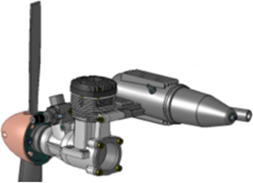
\includegraphics[width=.5\linewidth]{fig_00}}%figues de la page de garde


\iflivret
\pagestyle{empty}


%%%%%%%% PAGE DE GARDE COURS
\ifcours
% ==== BANDEAU DES TITRES ==== 
\begin{tikzpicture}[remember picture,overlay]
\node at (current page.north west)
{\begin{tikzpicture}[remember picture,overlay]
\node[anchor=north west,inner sep=0pt] at (0,0) {\includegraphics[width=\paperwidth]{\thechapterimage}};
\draw[anchor=west] (-2cm,-8cm) node [line width=2pt,rounded corners=15pt,draw=ocre,fill=white,fill opacity=0.6,inner sep=40pt]{\strut\makebox[22cm]{}};
\draw[anchor=west] (1cm,-8cm) node {\huge\sffamily\bfseries\color{black} %
\begin{minipage}{1cm}
\rotatebox{90}{\LARGE\sffamily\textsc{\color{ocre}\textbf{\xxnumpartie}}}
\end{minipage} \hfill
\begin{minipage}[c]{14cm}
\begin{titrepartie}
\begin{flushright}
\renewcommand{\baselinestretch}{1.1} 
\Large\sffamily\textsc{\textbf{\xxpartie}}
\renewcommand{\baselinestretch}{1} 
\end{flushright}
\end{titrepartie}
\end{minipage} \hfill
\begin{minipage}[c]{3.5cm}
{\large\sffamily\textsc{\textbf{\color{ocre} \discipline}}}
\end{minipage} 
 };
\end{tikzpicture}};
\end{tikzpicture}
% ==== FIN BANDEAU DES TITRES ==== 


% ==== ONGLET 
\begin{tikzpicture}[overlay]
\node[shape=rectangle, 
      rounded corners = .25 cm,
	  draw= ocre,
	  line width=2pt, 
	  fill = ocre!10,
	  minimum width  = 2.5cm,
	  minimum height = 3cm,] at (18.3cm,0) {};
\node at (17.7cm,0) {\rotatebox{90}{\textbf{\Large\color{ocre}{\classe}}}};
%{};
\end{tikzpicture}
% ==== FIN ONGLET 


\vspace{3.5cm}

\begin{tikzpicture}[remember picture,overlay]
\draw[anchor=west] (-2cm,-6cm) node {\huge\sffamily\bfseries\color{black} %
\begin{minipage}{2cm}
\begin{center}
\LARGE\sffamily\textsc{\color{ocre}\textbf{\xxactivite}}
\end{center}
\end{minipage} \hfill
\begin{minipage}[c]{15cm}
\begin{titrechapitre}
\renewcommand{\baselinestretch}{1.1} 
\Large\sffamily\textsc{\textbf{\xxnumchapitre}}

\Large\sffamily\textsc{\textbf{\xxchapitre}}
\vspace{.5cm}

\renewcommand{\baselinestretch}{1} 
\normalsize\normalfont
\xxcompetences
\end{titrechapitre}
\end{minipage}  };
\end{tikzpicture}
\vfill

\begin{flushright}
\begin{minipage}[c]{.3\linewidth}
\begin{center}
\xxfigures
\end{center}
\end{minipage}\hfill
\begin{minipage}[c]{.6\linewidth}
\startcontents
%\printcontents{}{1}{}
\printcontents{}{1}{}
\end{minipage}
\end{flushright}

\begin{tikzpicture}[remember picture,overlay]
\draw[anchor=west] (4.5cm,-.7cm) node {
\begin{minipage}[c]{.2\linewidth}
\begin{flushright}

\includegraphics[width=2cm]{logoCC}
\end{flushright}
\end{minipage}
\begin{minipage}[c]{.2\linewidth}
\textsl{\xxauteur} \\
\textsl{\classe}
\end{minipage}
 };
\end{tikzpicture}

\newpage
\pagestyle{fancy}

%\newpage
%\pagestyle{fancy}

\else
\fi
%% FIN PAGE DE GARDE DES COURS

%%%%%%%% PAGE DE GARDE TD
\iftd
%\begin{tikzpicture}[remember picture,overlay]
%\node at (current page.north west)
%{\begin{tikzpicture}[remember picture,overlay]
%\draw[anchor=west] (-2cm,-3.25cm) node [line width=2pt,rounded corners=15pt,draw=ocre,fill=white,fill opacity=0.6,inner sep=40pt]{\strut\makebox[22cm]{}};
%\draw[anchor=west] (1cm,-3.25cm) node {\huge\sffamily\bfseries\color{black} %
%\begin{minipage}{1cm}
%\rotatebox{90}{\LARGE\sffamily\textsc{\color{ocre}\textbf{\xxnumpartie}}}
%\end{minipage} \hfill
%\begin{minipage}[c]{13.5cm}
%\begin{titrepartie}
%\begin{flushright}
%\renewcommand{\baselinestretch}{1.1} 
%\Large\sffamily\textsc{\textbf{\xxpartie}}
%\renewcommand{\baselinestretch}{1} 
%\end{flushright}
%\end{titrepartie}
%\end{minipage} \hfill
%\begin{minipage}[c]{3.5cm}
%{\large\sffamily\textsc{\textbf{\color{ocre} \discipline}}}
%\end{minipage} 
% };
%\end{tikzpicture}};
%\end{tikzpicture}

%%%%%%%%%% PAGE DE GARDE TD %%%%%%%%%%%%%%%
%\begin{tikzpicture}[overlay]
%\node[shape=rectangle, 
%      rounded corners = .25 cm,
%	  draw= ocre,
%	  line width=2pt, 
%	  fill = ocre!10,
%	  minimum width  = 2.5cm,
%	  minimum height = 2.5cm,] at (18.5cm,0) {};
%\node at (17.7cm,0) {\rotatebox{90}{\textbf{\Large\color{ocre}{\classe}}}};
%%{};
%\end{tikzpicture}

% PARTIE ET CHAPITRE
%\begin{tikzpicture}[remember picture,overlay]
%\draw[anchor=west] (-1cm,-2.1cm) node {\large\sffamily\bfseries\color{black} %
%\begin{minipage}[c]{15cm}
%\begin{flushleft}
%\xxnumchapitre \\
%\xxchapitre
%\end{flushleft}
%\end{minipage}  };
%\end{tikzpicture}

% BANDEAU EXO
\iflivret % SI LIVRET
\begin{tikzpicture}[remember picture,overlay]
\draw[anchor=west] (-2cm,-3.3cm) node {\huge\sffamily\bfseries\color{black} %
\begin{minipage}{5cm}
\begin{center}
\LARGE\sffamily\color{ocre}\textbf{\textsc{\xxactivite}}

\begin{center}
\xxfigures
\end{center}

\end{center}
\end{minipage} \hfill
\begin{minipage}[c]{12cm}
\begin{titrechapitre}
\renewcommand{\baselinestretch}{1.1} 
\large\sffamily\textbf{\textsc{\xxtitreexo}}

\small\sffamily{\textbf{\textit{\color{black!70}\xxsourceexo}}}
\vspace{.5cm}

\renewcommand{\baselinestretch}{1} 
\normalsize\normalfont
\xxcompetences
\end{titrechapitre}
\end{minipage}};
\end{tikzpicture}
\else % ELSE NOT LIVRET
\begin{tikzpicture}[remember picture,overlay]
\draw[anchor=west] (-2cm,-4.5cm) node {\huge\sffamily\bfseries\color{black} %
\begin{minipage}{5cm}
\begin{center}
\LARGE\sffamily\color{ocre}\textbf{\textsc{\xxactivite}}

\begin{center}
\xxfigures
\end{center}

\end{center}
\end{minipage} \hfill
\begin{minipage}[c]{12cm}
\begin{titrechapitre}
\renewcommand{\baselinestretch}{1.1} 
\large\sffamily\textbf{\textsc{\xxtitreexo}}

\small\sffamily{\textbf{\textit{\color{black!70}\xxsourceexo}}}
\vspace{.5cm}

\renewcommand{\baselinestretch}{1} 
\normalsize\normalfont
\xxcompetences
\end{titrechapitre}
\end{minipage}};
\end{tikzpicture}

\fi

\else   % FIN IF TD
\fi


%%%%%%%% PAGE DE GARDE FICHE
\iffiche
\begin{tikzpicture}[remember picture,overlay]
\node at (current page.north west)
{\begin{tikzpicture}[remember picture,overlay]
\draw[anchor=west] (-2cm,-2.25cm) node [line width=2pt,rounded corners=15pt,draw=ocre,fill=white,fill opacity=0.6,inner sep=40pt]{\strut\makebox[22cm]{}};
\draw[anchor=west] (1cm,-2.25cm) node {\huge\sffamily\bfseries\color{black} %
\begin{minipage}{1cm}
\rotatebox{90}{\LARGE\sffamily\textsc{\color{ocre}\textbf{\xxnumpartie}}}
\end{minipage} \hfill
\begin{minipage}[c]{14cm}
\begin{titrepartie}
\begin{flushright}
\renewcommand{\baselinestretch}{1.1} 
\large\sffamily\textsc{\textbf{\xxpartie} \\} 

\vspace{.2cm}

\normalsize\sffamily\textsc{\textbf{\xxnumchapitre -- \xxchapitre}}
\renewcommand{\baselinestretch}{1} 
\end{flushright}
\end{titrepartie}
\end{minipage} \hfill
\begin{minipage}[c]{3.5cm}
{\large\sffamily\textsc{\textbf{\color{ocre} \discipline}}}
\end{minipage} 
 };
\end{tikzpicture}};
\end{tikzpicture}

\iflivret
\begin{tikzpicture}[overlay]
\node[shape=rectangle, 
      rounded corners = .25 cm,
	  draw= ocre,
	  line width=2pt, 
	  fill = ocre!10,
	  minimum width  = 2.5cm,
	  minimum height = 2.5cm,] at (18.5cm,.5cm) {};
\node at (17.9cm,.5cm) {\rotatebox{90}{\textsf{\textbf{\large\color{ocre}{\classe}}}}};
%{};
\end{tikzpicture}
\else
\begin{tikzpicture}[overlay]
\node[shape=rectangle, 
      rounded corners = .25 cm,
	  draw= ocre,
	  line width=2pt, 
	  fill = ocre!10,
	  minimum width  = 2.5cm,
%	  minimum height = 2.5cm,] at (18.5cm,1.1cm) {};
	  minimum height = 2.5cm,] at (18.6cm,0.5cm) {};
\node at (18cm,0.5cm) {\rotatebox{90}{\textsf{\textbf{\large\color{ocre}{\classe}}}}};
%{};
\end{tikzpicture}

\fi

\else
\fi



\else
\pagestyle{empty}


%%%%%%%% PAGE DE GARDE COURS
\ifcours
% ==== BANDEAU DES TITRES ==== 
\begin{tikzpicture}[remember picture,overlay]
\node at (current page.north west)
{\begin{tikzpicture}[remember picture,overlay]
\node[anchor=north west,inner sep=0pt] at (0,0) {\includegraphics[width=\paperwidth]{\thechapterimage}};
\draw[anchor=west] (-2cm,-8cm) node [line width=2pt,rounded corners=15pt,draw=ocre,fill=white,fill opacity=0.6,inner sep=40pt]{\strut\makebox[22cm]{}};
\draw[anchor=west] (1cm,-8cm) node {\huge\sffamily\bfseries\color{black} %
\begin{minipage}{1cm}
\rotatebox{90}{\LARGE\sffamily\textsc{\color{ocre}\textbf{\xxnumpartie}}}
\end{minipage} \hfill
\begin{minipage}[c]{14cm}
\begin{titrepartie}
\begin{flushright}
\renewcommand{\baselinestretch}{1.1} 
\Large\sffamily\textsc{\textbf{\xxpartie}}
\renewcommand{\baselinestretch}{1} 
\end{flushright}
\end{titrepartie}
\end{minipage} \hfill
\begin{minipage}[c]{3.5cm}
{\large\sffamily\textsc{\textbf{\color{ocre} \discipline}}}
\end{minipage} 
 };
\end{tikzpicture}};
\end{tikzpicture}
% ==== FIN BANDEAU DES TITRES ==== 


% ==== ONGLET 
\begin{tikzpicture}[overlay]
\node[shape=rectangle, 
      rounded corners = .25 cm,
	  draw= ocre,
	  line width=2pt, 
	  fill = ocre!10,
	  minimum width  = 2.5cm,
	  minimum height = 3cm,] at (18.3cm,0) {};
\node at (17.7cm,0) {\rotatebox{90}{\textbf{\Large\color{ocre}{\classe}}}};
%{};
\end{tikzpicture}
% ==== FIN ONGLET 


\vspace{3.5cm}

\begin{tikzpicture}[remember picture,overlay]
\draw[anchor=west] (-2cm,-6cm) node {\huge\sffamily\bfseries\color{black} %
\begin{minipage}{2cm}
\begin{center}
\LARGE\sffamily\textsc{\color{ocre}\textbf{\xxactivite}}
\end{center}
\end{minipage} \hfill
\begin{minipage}[c]{15cm}
\begin{titrechapitre}
\renewcommand{\baselinestretch}{1.1} 
\Large\sffamily\textsc{\textbf{\xxnumchapitre}}

\Large\sffamily\textsc{\textbf{\xxchapitre}}
\vspace{.5cm}

\renewcommand{\baselinestretch}{1} 
\normalsize\normalfont
\xxcompetences
\end{titrechapitre}
\end{minipage}  };
\end{tikzpicture}
\vfill

\begin{flushright}
\begin{minipage}[c]{.3\linewidth}
\begin{center}
\xxfigures
\end{center}
\end{minipage}\hfill
\begin{minipage}[c]{.6\linewidth}
\startcontents
%\printcontents{}{1}{}
\printcontents{}{1}{}
\end{minipage}
\end{flushright}

\begin{tikzpicture}[remember picture,overlay]
\draw[anchor=west] (4.5cm,-.7cm) node {
\begin{minipage}[c]{.2\linewidth}
\begin{flushright}

\includegraphics[width=2cm]{logoCC}
\end{flushright}
\end{minipage}
\begin{minipage}[c]{.2\linewidth}
\textsl{\xxauteur} \\
\textsl{\classe}
\end{minipage}
 };
\end{tikzpicture}

\newpage
\pagestyle{fancy}

%\newpage
%\pagestyle{fancy}

\else
\fi
%% FIN PAGE DE GARDE DES COURS

%%%%%%%% PAGE DE GARDE TD
\iftd
%\begin{tikzpicture}[remember picture,overlay]
%\node at (current page.north west)
%{\begin{tikzpicture}[remember picture,overlay]
%\draw[anchor=west] (-2cm,-3.25cm) node [line width=2pt,rounded corners=15pt,draw=ocre,fill=white,fill opacity=0.6,inner sep=40pt]{\strut\makebox[22cm]{}};
%\draw[anchor=west] (1cm,-3.25cm) node {\huge\sffamily\bfseries\color{black} %
%\begin{minipage}{1cm}
%\rotatebox{90}{\LARGE\sffamily\textsc{\color{ocre}\textbf{\xxnumpartie}}}
%\end{minipage} \hfill
%\begin{minipage}[c]{13.5cm}
%\begin{titrepartie}
%\begin{flushright}
%\renewcommand{\baselinestretch}{1.1} 
%\Large\sffamily\textsc{\textbf{\xxpartie}}
%\renewcommand{\baselinestretch}{1} 
%\end{flushright}
%\end{titrepartie}
%\end{minipage} \hfill
%\begin{minipage}[c]{3.5cm}
%{\large\sffamily\textsc{\textbf{\color{ocre} \discipline}}}
%\end{minipage} 
% };
%\end{tikzpicture}};
%\end{tikzpicture}

%%%%%%%%%% PAGE DE GARDE TD %%%%%%%%%%%%%%%
%\begin{tikzpicture}[overlay]
%\node[shape=rectangle, 
%      rounded corners = .25 cm,
%	  draw= ocre,
%	  line width=2pt, 
%	  fill = ocre!10,
%	  minimum width  = 2.5cm,
%	  minimum height = 2.5cm,] at (18.5cm,0) {};
%\node at (17.7cm,0) {\rotatebox{90}{\textbf{\Large\color{ocre}{\classe}}}};
%%{};
%\end{tikzpicture}

% PARTIE ET CHAPITRE
%\begin{tikzpicture}[remember picture,overlay]
%\draw[anchor=west] (-1cm,-2.1cm) node {\large\sffamily\bfseries\color{black} %
%\begin{minipage}[c]{15cm}
%\begin{flushleft}
%\xxnumchapitre \\
%\xxchapitre
%\end{flushleft}
%\end{minipage}  };
%\end{tikzpicture}

% BANDEAU EXO
\iflivret % SI LIVRET
\begin{tikzpicture}[remember picture,overlay]
\draw[anchor=west] (-2cm,-3.3cm) node {\huge\sffamily\bfseries\color{black} %
\begin{minipage}{5cm}
\begin{center}
\LARGE\sffamily\color{ocre}\textbf{\textsc{\xxactivite}}

\begin{center}
\xxfigures
\end{center}

\end{center}
\end{minipage} \hfill
\begin{minipage}[c]{12cm}
\begin{titrechapitre}
\renewcommand{\baselinestretch}{1.1} 
\large\sffamily\textbf{\textsc{\xxtitreexo}}

\small\sffamily{\textbf{\textit{\color{black!70}\xxsourceexo}}}
\vspace{.5cm}

\renewcommand{\baselinestretch}{1} 
\normalsize\normalfont
\xxcompetences
\end{titrechapitre}
\end{minipage}};
\end{tikzpicture}
\else % ELSE NOT LIVRET
\begin{tikzpicture}[remember picture,overlay]
\draw[anchor=west] (-2cm,-4.5cm) node {\huge\sffamily\bfseries\color{black} %
\begin{minipage}{5cm}
\begin{center}
\LARGE\sffamily\color{ocre}\textbf{\textsc{\xxactivite}}

\begin{center}
\xxfigures
\end{center}

\end{center}
\end{minipage} \hfill
\begin{minipage}[c]{12cm}
\begin{titrechapitre}
\renewcommand{\baselinestretch}{1.1} 
\large\sffamily\textbf{\textsc{\xxtitreexo}}

\small\sffamily{\textbf{\textit{\color{black!70}\xxsourceexo}}}
\vspace{.5cm}

\renewcommand{\baselinestretch}{1} 
\normalsize\normalfont
\xxcompetences
\end{titrechapitre}
\end{minipage}};
\end{tikzpicture}

\fi

\else   % FIN IF TD
\fi


%%%%%%%% PAGE DE GARDE FICHE
\iffiche
\begin{tikzpicture}[remember picture,overlay]
\node at (current page.north west)
{\begin{tikzpicture}[remember picture,overlay]
\draw[anchor=west] (-2cm,-2.25cm) node [line width=2pt,rounded corners=15pt,draw=ocre,fill=white,fill opacity=0.6,inner sep=40pt]{\strut\makebox[22cm]{}};
\draw[anchor=west] (1cm,-2.25cm) node {\huge\sffamily\bfseries\color{black} %
\begin{minipage}{1cm}
\rotatebox{90}{\LARGE\sffamily\textsc{\color{ocre}\textbf{\xxnumpartie}}}
\end{minipage} \hfill
\begin{minipage}[c]{14cm}
\begin{titrepartie}
\begin{flushright}
\renewcommand{\baselinestretch}{1.1} 
\large\sffamily\textsc{\textbf{\xxpartie} \\} 

\vspace{.2cm}

\normalsize\sffamily\textsc{\textbf{\xxnumchapitre -- \xxchapitre}}
\renewcommand{\baselinestretch}{1} 
\end{flushright}
\end{titrepartie}
\end{minipage} \hfill
\begin{minipage}[c]{3.5cm}
{\large\sffamily\textsc{\textbf{\color{ocre} \discipline}}}
\end{minipage} 
 };
\end{tikzpicture}};
\end{tikzpicture}

\iflivret
\begin{tikzpicture}[overlay]
\node[shape=rectangle, 
      rounded corners = .25 cm,
	  draw= ocre,
	  line width=2pt, 
	  fill = ocre!10,
	  minimum width  = 2.5cm,
	  minimum height = 2.5cm,] at (18.5cm,.5cm) {};
\node at (17.9cm,.5cm) {\rotatebox{90}{\textsf{\textbf{\large\color{ocre}{\classe}}}}};
%{};
\end{tikzpicture}
\else
\begin{tikzpicture}[overlay]
\node[shape=rectangle, 
      rounded corners = .25 cm,
	  draw= ocre,
	  line width=2pt, 
	  fill = ocre!10,
	  minimum width  = 2.5cm,
%	  minimum height = 2.5cm,] at (18.5cm,1.1cm) {};
	  minimum height = 2.5cm,] at (18.6cm,0.5cm) {};
\node at (18cm,0.5cm) {\rotatebox{90}{\textsf{\textbf{\large\color{ocre}{\classe}}}}};
%{};
\end{tikzpicture}

\fi

\else
\fi



\fi
\setlength{\columnseprule}{.1pt}

\pagestyle{fancy}
\thispagestyle{plain}

\ifprof
\vspace{5.1cm}
\else
\vspace{5.2cm}
\fi

\def\columnseprulecolor{\color{ocre}}
\setlength{\columnseprule}{0.4pt} 

%%%%%%%%%%%%%%%%%%%%%%%

\setcounter{exo}{0}



\ifprof
\else
\begin{multicols}{2}
\fi

\subsection*{Mise en situation}

\ifprof
\else
Le développement de robots à forme humaine est en
croissance constante depuis quelques dizaines
d’années. En robotique, il est difficile d’affirmer que
tous les robots remplaçant l’homme dans ses tâches
doivent être de forme humaine. Les véhicules
autonomes, par exemple, ne sont pas
anthropomorphes. Les tâches auxquelles sont
destinées les robots définissent leur forme idéale. Si
nous souhaitons un jour que les robots remplacent
l’homme dans ses tâches ennuyeuses, ils devront
s’intégrer au mieux à notre société, à notre
environnement et à notre ergonomie.

Les dimensions d’une maison et la hauteur des meubles sont adaptées à notre forme humaine. L’avantage
des robots humanoïdes devient alors économique : il n’est pas indispensable de modifier l’environnement
quotidien pour les utiliser.

Le robot humanoïde LOLA, développé par l’Université de Munich, est un robot de forme humaine
conçu pour un mode de marche rapide. LOLA possède une structure à 25 degrés de liberté lui permettant une
flexibilité accrue. Chaque jambe possède 7 degrés de liberté, le haut du corps 8 et la tête 3.
Le robot est équipé d’une caméra stéréoscopique haute définition afin de percevoir son environnement, d’une
centrale inertielle équipée de 3 gyroscopes et de 3 accéléromètres. Chaque articulation possède un codeur
angulaire absolu et chaque pied est muni d’un capteur d’effort 6 axes permettant d’obtenir l’effort de contact
avec le sol. Les caractéristiques techniques de LOLA sont données dans le tableau suivant.


\begin{center}
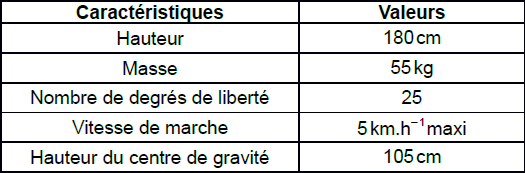
\includegraphics[width=\linewidth]{fig_01_a}
\end{center}
\fi

\subsection*{Stabilité du robot}
\ifprof
\else

Par définition, le robot humanoïde bipède s'appuie sur ses deux jambes.
Comme tout système de solides en équilibre statique, LOLA est à l’équilibre si
la projection de son centre de gravité sur le sol est contenu dans le polygone
de sustentation qui est tracé en rouge autour de ses deux pieds sur la figure suivante.
Lorsque le robot marche, il y a une phase où il n'est en appui que sur un seul
pied. Dans ce cas, le polygone de sustentation est réduit à un seul pied.


\begin{center}
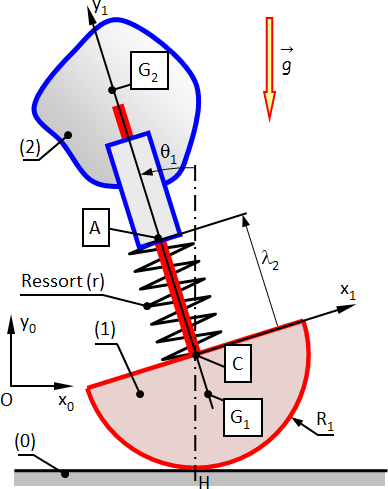
\includegraphics[width=.5\linewidth]{fig_01}
\end{center}
\fi
\begin{obj}
L’objectif de cette partie est de trouver à quelle condition le maintien du contact sur le sol est possible lorsque
le robot marche et si l'accélération est compatible avec le cahier des charges, dont un extrait est donné ciaprès.
\end{obj}

\begin{center}
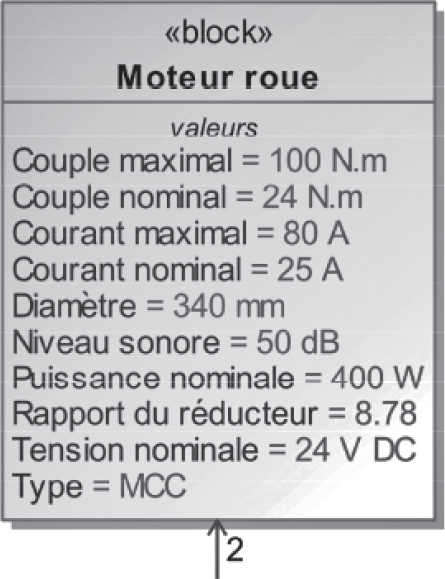
\includegraphics[width=\linewidth]{fig_02}
\end{center}


\ifprof
\else

Le contact du pied sur le sol est modélisé sans frottement sur la figure suivante.


\begin{center}
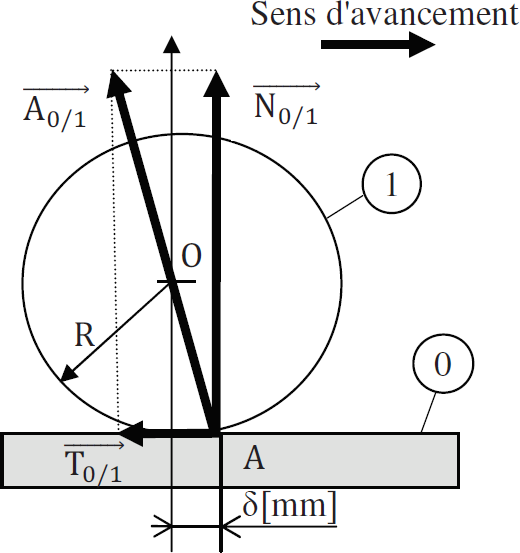
\includegraphics[width=\linewidth]{fig_03}
\end{center}
\fi

\subsection*{Modélisation de l’effort de contact entre le sol et le robot}

\ifprof
\else

Sous la semelle du robot, la pression de contact avec le sol est supposée répartie de manière uniforme
transversalement (suivant la direction $\vect{x_0}$). Le problème se ramène donc à une répartition linéique de pression
sur les deux segments de contact $[O_S ;A_S]$ et $[B_S;C_S]$ . En chaque point $M$ (d'ordonnée $\vect{y}$) de ces
segments, la densité d'efforts de contact est $p(M)\vect{z_0}$ , avec $p(M)$ en $\text{N m}^{-2}$. On notera que si le robot n'est pas équipé de semelles magnétiques ou adhésives, on a $p(M)> 0$. Ainsi, en notant $b$ la largeur de la semelle
suivant$\vect{x_0}$ et $\Sigma=[O_S ,A_S]\cup [B_S,C_S]$, le modèle global d'action mécanique de contact du sol sur le pied peut être donné par le torseur :
$
\torseurstat{T}{\text{sol}}{\text{pied}}=\torseurl{\vectf{\text{sol}}{\text{pied}}=b\int_{M\in\Sigma} p(M)\vect{z_0} \dd y }{\vectm{O_S}{\text{sol}}{\text{pied}}=b\int_{M\in\Sigma} \vect{O_S M} \wedge p(M)\vect{z_0} \dd {y}}{O_S}$.

\fi

\subparagraph{} \textit{Montrer que $\torseurstat{T}{\text{sol}}{\text{pied}}$ est un glisseur.}
\ifprof
\begin{corrige}~\\
L'automoment est un des invariants du torseur : $\forall P, \vectf{\text{sol}}{\text{pied}}\cdot\vectm{O_S}{\text{sol}}{\text{pied}}=\text{cst}$. Dans le cas d'un glisseur, il existe un point tel que le moment est nul. L'automoment est donc nul en tous points de l'espace.

Dans notre cas, $b\int_{M\in\Sigma} p(M)\vect{z_0} \dd y \cdot b\int_{M\in\Sigma} \vect{O_S M} \wedge p(M)\vect{z_0} \dd y = 0$ (permutation circulaire du produit mixte). 


 
\end{corrige}
\else
\fi

\ifprof
\else

Soit $H_S$ le point de la droite $\left(O_S,\vect{y_0}\right)$ tel que  
$\vectm{H_S}{\text{sol}}{\text{pied}}=\vect{0}$, on notera $\vect{O_SH_S} = Y_{H_S}\vect{y_0}$. Ce point est
fondamental en robotique humanoïde, il prend le nom de Zero Moment Point (ZMP) : de l'anglais « point de
moment nul ».

\fi


\subparagraph{} \textit{Montrer que $H_S\in [O_S;C_S]$, c'est à-dire qu'il est situé sous le pied du robot.}
\ifprof
\begin{corrige}
On a $   \vectm{H_S}{\text{sol}}{\text{pied}} =\vect{0}$.

D'une part,  $\vectm{O_S}{\text{sol}}{\text{pied}} =  \vectm{H_S}{\text{sol}}{\text{pied}} + \vect{ O_SH_S} \wedge \vectf{\text{sol}}{\text{pied}}$

$\Leftrightarrow  \int_{M\in\Sigma} \vect{O_S M} \wedge p(M)\vect{z_0} \dd {y}=   \vect{ O_SH_S} \wedge \int_{M\in\Sigma} p(M)\vect{z_0} \dd y$

$\Leftrightarrow \int_{M\in\Sigma} \lambda \vect{y_0} \wedge p(M)\vect{z_0} \dd {y}=   L_1 \vect{y_0} \wedge \int_{M\in\Sigma} p(M)\vect{z_0} \dd y$

$\Leftrightarrow  \int_{M\in\Sigma}\lambda  p(M) \dd {y}=   L_1  \int_{M\in\Sigma} p(M) \dd y$

$\Leftrightarrow L_1 = \dfrac{\int_{M\in\Sigma}\lambda  p(M) \dd {y}}{  \int_{M\in\Sigma} p(M) \dd y}$

D'autre part,  $\vectm{C_S}{\text{sol}}{\text{pied}} =  \vectm{H_S}{\text{sol}}{\text{pied}} + \vect{ C_SH_S} \wedge \vectf{\text{sol}}{\text{pied}}$

$\Leftrightarrow  \int_{M\in\Sigma} \vect{O_S M} \wedge p(M)\vect{z_0} \dd {y}=  \vect{ C_SH_S}  \wedge \int_{M\in\Sigma} p(M)\vect{z_0} \dd y$

$\Leftrightarrow  \int_{M\in\Sigma} \lambda \vect{y_0} \wedge p(M)\vect{z_0} \dd {y}=  L_2 \vect{y_0}   \wedge \int_{M\in\Sigma} p(M)\vect{z_0} \dd y$


$\Leftrightarrow  \int_{M\in\Sigma} \lambda  p(M)\dd {y}=  L_2   \int_{M\in\Sigma} p(M) \dd y$

$\Leftrightarrow L_2 =  \dfrac{\int_{M\in\Sigma} \lambda  p(M)\dd {y} }{ \int_{M\in\Sigma} p(M) \dd y}  $

%
%On cherche $H_S$ tel que $   \vectm{H_S}{\text{sol}}{\text{pied}} =  \vectm{O_S}{\text{sol}}{\text{pied}}   + \vect{H_S O_S} \wedge \vectf{\text{sol}}{\text{pied}} = \vect{0} $ 
%soit 
%$ \vectm{O_S}{\text{sol}}{\text{pied}}   + \vect{H_S O_S} \wedge \vectf{\text{sol}}{\text{pied}} = \vect{0}$
%
%$ b\int_{M\in\Sigma} \vect{O_S M} \wedge p(M)\vect{z_0} \dd {y}  + \vect{H_S O_S} \wedge b\int_{M\in\Sigma} p(M)\vect{z_0} \dd y = \vect{0}$
%
%$\Leftrightarrow  \int_{M\in\Sigma} \vect{O_S M} \wedge p(M)\vect{z_0} \dd {y}  + \vect{H_S O_S} \wedge \int_{M\in\Sigma} p(M)\vect{z_0} \dd y = \vect{0}$
%
%$\Leftrightarrow  \int_{M\in\Sigma} \left( \vect{O_S M} \wedge p(M)\vect{z_0}  + \vect{H_S O_S} \wedge p(M)\vect{z_0} \right) \dd {y}   = \vect{0}$
%
%$\Leftrightarrow  \int_{M\in\Sigma} \left( \vect{O_S M}  + \vect{H_S O_S} \right) \wedge p(M)\vect{z_0}  \dd {y}   = \vect{0}$
%
%$\Leftrightarrow  \int_{M\in\Sigma}   \vect{H_S M}  \wedge p(M)\vect{z_0}  \dd {y}   = \vect{0}$

\end{corrige}
\else
\fi



\subparagraph{} \textit{Donner la forme du torseur $\torseurstat{T}{\text{sol}}{\text{pied}}$ dans le cas d'un contact avec frottement dans le plan sagittal (c'est-à dire que la densité d'efforts de contact est $p(M)\vect{z_0}+t(M)\vect{y_0}$ ). Montrer que les résultats des questions 1 et 2 sont inchangés.}
\ifprof
\begin{corrige}
$
\torseurstat{T}{\text{sol}}{\text{pied}}=\torseurl{b\int_{M\in\Sigma}\left(p(M)\vect{z_0}+t(M)\vect{y_0}\right) \dd y }{b\int_{M\in\Sigma} \vect{O_S M} \wedge p(M)\vect{z_0} \dd {y}}{O_S}$

$=\torseurl{b\int_{M\in\Sigma}p(M)\vect{z_0}\dd y }{b\int_{M\in\Sigma} \vect{O_S M} \wedge p(M)\vect{z_0} \dd {y}}{O_S}+\torseurl{b\int_{M\in\Sigma}t(M)\vect{y_0}\dd y }{\vect{0}}{O_S}$.

Le premier torseur vérifie bien les deux premières questions. Le second torseur est bien un glisseur (automoment nul). 

(...)


\end{corrige}
\else
\fi

\subsection*{Établissement de la condition de non-basculement}
\ifprof
\else

Considérons le robot en marche avec le torse ayant un mouvement de
translation vers l’avant (suivant $+\vect{y_0}$). Le robot est toujours dans la
phase d'appui d'un seul pied sur le sol, via une des deux jambes notées
(2).

Données et paramètres :
\begin{itemize}
\item Torse (1) :
\begin{itemize}
\item masse $m_1$, accélération de la pesanteur : $\vect{g}=-g\vect{z_0}$ avec
$g=\SI{9,81}{m.s^{-2}}$;
\item centre de gravité : $G$, tel que $\vect{O_SG}=Y_G(t)\vect{y_0}+Z_G(t)\vect{z_0}$;
\item le torse est supposé en mouvement de translation rectiligne, de direction $\vect{y_0}$ par rapport au sol, on a : $\torseurcin{V}{1}{\text{Sol}}=\torseurl{\vect{0}}{\dfrac{\dd Y_G}{\dd t}\vect{y_0}}{G}$.
\end{itemize}
\item Jambe avec les pieds (2) :
\begin{itemize}
\item masses et inerties négligeables dans cette phase;
\item le pied d'appui est sans mouvement par rapport au sol;
\item l'action mécanique du sol sur la semelle du pied est modélisée par le glisseur : $\torseurstat{T}{\text{sol}}{\text{pied}}=\torseurl{\vectf{\text{sol}}{\text{pied}}}{\vect{0}}{H_S}$
où : $H_S$ est le ZMP, point mis en évidence à la question 2 tel que $\vect{O_S H_S}=Y_{H_S}\vect{y_0}$, 
 $\vectf{\text{sol}}{\text{pied}}=N_{\text{sol}\rightarrow \text{pied}}\vect{z_0}+T_{\text{sol}\rightarrow \text{pied}}\vect{y_0}$, avec à la limite du glissement $\left| T_{\text{sol}\rightarrow \text{pied}}\right| = \mu N_{\text{sol}\rightarrow \text{pied}}$ où $\mu$ est le facteur de frottement du contact sol / semelle.
\end{itemize}
\end{itemize}

\begin{center}
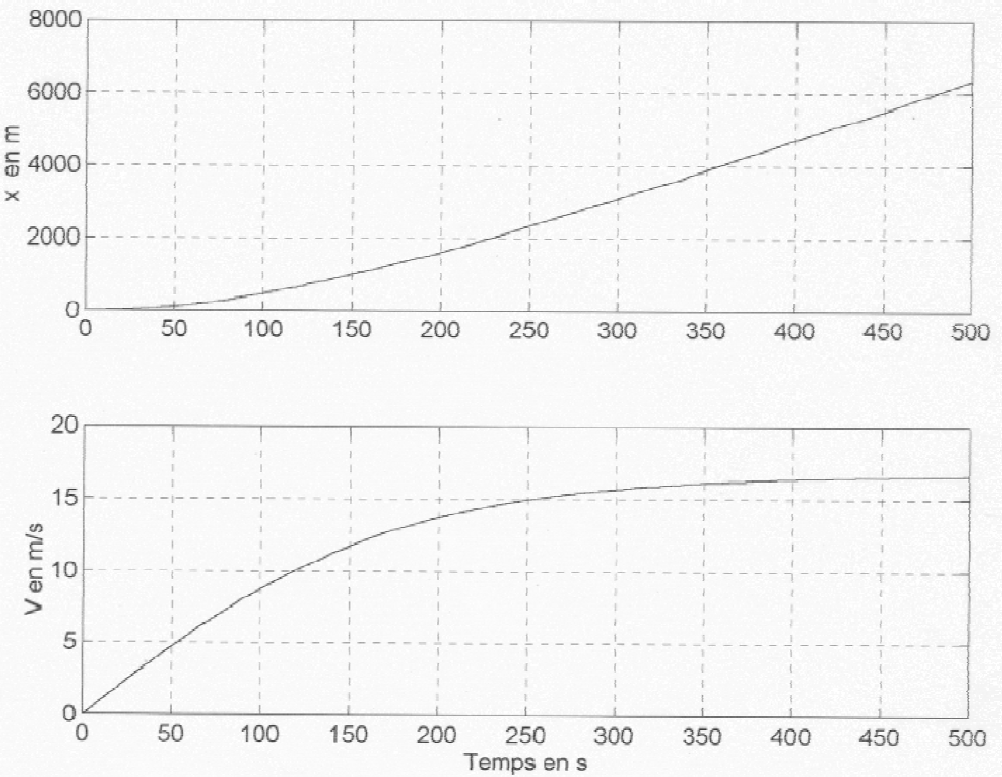
\includegraphics[width=.4\linewidth]{fig_04}
\end{center}
\fi

\subparagraph{} \textit{En appliquant le théorème du moment dynamique, puis le théorème de la résultante dynamique au
système \{1+2\}, montrer que la condition de stabilité (non basculement) s'écrit : $Y_{H_S}=Y_G-\dfrac{Z_G}{g}\dfrac{\dd^2 Y_G}{\dd t^2}$.}
\ifprof
\begin{corrige} ~\\

\begin{center}
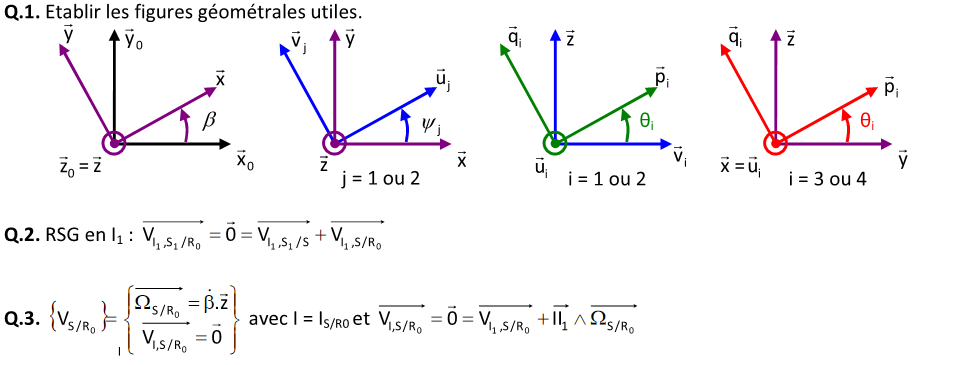
\includegraphics[width=.5\linewidth]{cor_01}
\end{center}

\begin{itemize}
\item On isole 1+2.
\item Bilan des actions mécaniques :
\begin{itemize}
\item action de la pesanteur;
\item action du sol.
\end{itemize}
\item On applique le TMD au point $H_S$ en projection sur $\vect{y_0}$. 
\begin{itemize}
\item $\vectmd{1}{0}{G}=\vect{0}$ (mouvement de translation). $\vectmd{1}{0}{H_S}=\vectmd{1}{0}{G}+\vect{H_S G}\wedge \vectrd{1}{0}$ 

$=m_1\left(-Y_{H_S}\vect{y_0}+Y_G(t)\vect{y_0}+Z_G(t)\vect{z_0}\right) \wedge \ddot{Y}_G\vect{y_0}$
$=-m_1Z_G(t) \ddot{Y}_G\vect{x_0}$.

\item Déplacement de l'action de la pesanteur : $\left(-Y_{H_S}\vect{y_0}+Y_G(t)\vect{y_0}+Z_G(t)\vect{z_0}\right) \wedge - m_1 g \vect{z_0} $

  $= - m_1 g \left(-Y_{H_S}\vect{x_0}+Y_G(t)\vect{x_0}\right) $.
  \item Au final, $- m_1 g \left(-Y_{H_S}+Y_G(t)\right) = -m_1Z_G(t) \ddot{Y}_G$ 
  $\Leftrightarrow   g \left(-Y_{H_S}+Y_G(t)\right) = Z_G(t) \ddot{Y}_G$. On a donc $gY_G(t)- Z_G(t) \ddot{Y}_G=gY_{H_S}$ et $Y_{H_S} = \dfrac{gY_G(t)- Z_G(t) \ddot{Y}_G}{g}$.
\end{itemize}
\end{itemize}

En faisant le TMD au point $H_S$ il est inutile de faire le TRD. 
\end{corrige}
\else
\fi


\ifprof
\else

Conformément au résultat de la question 2, le calculateur du robot contrôle en permanence la position du
point $H_S$ (ZMP) : s'il est positionné à l'intérieur du segment $[O_S ;C_S ]$, le robot ne bascule pas.
On appelle foulée, la longueur entre deux emplacements successifs d'appui du même pied. Lors du premier
pas, le centre de gravité se déplace de sorte que $Y_G \in \left[ -\dfrac{\text{foulee}}{4},+\dfrac{\text{foulee}}{4}\right]$, car pour une accélération constante, les deux pas qui constituent une foulée sont de même longueur.

Le cahier des charges stipule qu'à partir de la station immobile, le robot doit atteindre la vitesse cible de \SI{5}{kmh^{-1}} en une seconde, avec une accélération constante du centre de gravité $\dfrac{\dd^2 Y_G}{\dd t^2}=\SI{1,39}{m.s^{-2}}$.
On rappelle que $Z_G=\SI{105}{cm}$.

\fi


\subparagraph{} \textit{Sachant que la longueur de la semelle du robot $[O_S ;C_S]$ est $L=\SI{300}{mm}$, déterminez la longueur de la première foulée du robot qui garantit la condition de non-basculement. Est-ce compatible avec le
cahier des charges ?}
\ifprof
\begin{corrige}
Le cas limite de basculement est lorsque $H_S=C_S$ et donc $Y_{H_S}=L$. 

On a donc $Y_G(t) = Y_{H_S} + \dfrac{ Z_G(t) \ddot{Y}_G}{g} = 300+\dfrac{1050\times1390}{9 810} = \SI{449}{mm} $.

La foulée est donnée par $4Y_G\simeq  \SI{1,795}{m}<\SI{1,50}{m}$. L'exigence 1.1.4 n'est pas respectée.
\end{corrige}
\else
\fi



\subparagraph{} \textit{Dans le cas d'un sol relativement glissant, avec un facteur de frottement du contact sol/semelle
$\mu =0,1$, quelle accélération maximale $\left[\dfrac{\dd^2 Y_G(t)}{\dd t^2}\right]_{\text{max}}$ 
le robot peut-il avoir ? Est-ce compatible avec le
cahier des charges pour la phase de démarrage ?}
\ifprof
\begin{corrige}

On isole (1+2) et on réalise le TRD :
\begin{itemize}
\item projection sur $\vect{y_0}$ : $b\int_{M\in\Sigma}t(M) \dd y= m_1 \dfrac{\dd^2 Y_G(t)}{\dd t^2}$;

\item projection sur $\vect{z_0}$ : $b\int_{M\in\Sigma}p(M) \dd y - m_1 g  = 0$.
\end{itemize}

À la limite du glissement, on a $b\int_{M\in\Sigma}t(M) \dd y= \mu b\int_{M\in\Sigma}p(M) \dd y$ soit 
$\left[\dfrac{\dd^2 Y_G(t)}{\dd t^2}\right]_{\text{max}} = \mu  g = 0,1\times 9,81 = \SI{0,981}{m.s^{-2}} < \SI{1,39}{m.s^{-2}}$. L'exigence 1.1.3 n'est pas respectée. 
\end{corrige}
\else
\fi



\ifprof
\else
\end{multicols}
\fi

